\documentclass{article}

\usepackage[english]{babel}

\usepackage[a4paper,top=2cm,bottom=2cm,left=3cm,right=3cm,marginparwidth=1.75cm]{geometry}

\usepackage{amsmath}
\usepackage{graphicx}
\usepackage[colorlinks=true, allcolors=blue]{hyperref}

\newcounter{eqn}
\renewcommand*{\theeqn}{\alph{eqn})}
\newcommand{\num}{\refstepcounter{eqn}\text{\theeqn}\;}

\makeatletter
\newcommand{\putindeepbox}[2][0.7\baselineskip]{{%
    \setbox0=\hbox{#2}%
    \setbox0=\vbox{\noindent\hsize=\wd0\unhbox0}
    \@tempdima=\dp0
    \advance\@tempdima by \ht0
    \advance\@tempdima by -#1\relax
    \dp0=\@tempdima
    \ht0=#1\relax
    \box0
}}
\makeatother

\title{GPU-Accelerated CFD Simulation of Downburst Effects on Buildings}
\author{Lucas Fonseca Timm}

\begin{document}
\maketitle

\newpage
\begin{abstract}
Your abstract.
\end{abstract}

\section{Introduction}
A downburst is a strong descending wind that impinges on the surface, forming one or multiple toroidal vortices that travel radially outward \cite{canepa}\cite{zhang}. They were first classified by Fujita\cite{fujita} in 1985 and were split into two major categories, differing by their sizes: "microburst" ($\leq 4\ km$) and "macroburst" ($> 4\ km$). Downbursts are generated by strong convective weather \cite{zhang} and have posed difficulties for study because they are limited to small regions and for a short period of time \cite{mason2009} \cite{aboshosha2015} \cite{mejia2022} \cite{yao2024} \cite{solari2020}. Despite brevity, they generate strong winds, with both horizontal and vertical components just above the surface, around $50m$ \cite{kim} \cite{aboshosha2015}. Building standards or design codes, written with the atmospheric boundary layer (ABL) in mind, usually do not consider \cite{chay} \cite{sengupta}.

Studying the effects of downbursts is essential, especially for light and low-rise structures, such as transmission towers and grain silos and industrial buildings or warehouses, that might fail during extreme weather and severe winds\cite{zhang2014}. As cited by Abd-Elaal et al.\cite{sayed}, 90\% of total damage and failure of transmission towers are attributed to downburst events rather than other types of thunderstorms. 


\subsection{Different Modeling Methods}
Due to the different flow geometry and velocity magnitude between downbursts and ABL, wind tunnels cannot easily reproduce microbursts nor macrobursts, and as such, different modeling methods have been used to simulate the effects of downbursts, both numerically and experimentally. Of note for the present study are: impinging jet (IJ) and cooling source (CS) \cite{zhang2}\cite{solari2020}. IJ, which was used for this work, is simple to model and build, and has been widely used \cite{solari2020}, while CS is harder to accomplish experimentally, but can be used numerically with the introduction of a cooling function \cite{zhang2}. 

\subsection{Numerical Procedures For Downburst Simulation}
Numerical methods are prevalent in downburst study \cite{aboshosha2015} \cite{chay} \cite{chen2007} \cite{kim} \cite{li2012} \cite{mason2009} \cite{mason2010} \cite{proctor1988} \cite{proctor1989} \cite{selvam1992} \cite{vermeire2011cooling} \cite{vermeire2011outflows} \cite{yao2024} \cite{zuzul2024} \cite{haines2018} \cite{sengupta} \cite{sengupta2008loads} \cite{wood2001} \cite{yan2022}. Through Computational Fluid Dynamics (CFD), it is possible even for modest workstations to simulate the IJ model in a reasonable amount of time. Modern approaches rely on parallelism as much as possible, and through the use of graphics processing units (GPU), it is possible to accelerate the simulation process and achieve speedups, the relationship between serial and parallel applications, unimaginable by past standards of performance. This happens because, although transistor counts have continued doubling in the past decades, per Moore's Law, single-core frequency in CPUs has not followed suit \cite{zenodo}. As such, improvements in high-performance computing (HPC) for science and engineering have come from leveraging multi-core and massively parallel architectures, in CPUs and GPUs respectively.

In past works proprietary software, such as Ansys Fluent, was used to model the IJ \cite{kim} [more citations]. Ansys Fluent is not GPU-accelerated by default, and to access the full performance gain of GPUs in it a enterprise license is required. Free and open-source alternatives exist, such as OpenFOAM, which do support some GPU Acceleration via third-party projects. However for this work a CFD program based on Braun's \cite{braun} proposed numerical procedure was used for simulating the downburst, the specific numerical setup will be described in section \ref{cfdsetup}. The program uses NVIDIA's  CUDA platform to access the GPU in the Fortran Programming Language, through the HPC SDK's \textit{nvfortran} compiler. Simulations were run both on a domestic workstation, hosting a RTX 3060, and in a HPC cluster made available by the Informatics Institute at UFRGS (Inf): \textit{PCAD} (High Performance Computing Cluster) has gpu-enabled compute nodes, between them, \textit{tupi} was chosen to run experiments due to having a more modern RTX 4090 available.

\subsection{Goals and Project Structure}
  In this work, a low-rise structure, represented as a rigid cube is going to be simulated both under ABL and downburstm, using the IJ model, drag and lift coefficients as well as the overall pressure distribution will be recorded and compared between the two different wind cases. Meshes will be generated by \textit{gmsh}, an open-source finite element mesh generation software, and analyzed later through \textit{Paraview}, an open-source scientific visualization tool. Computationally, performance analysis on the gpu program will be done using the tools provided by NVIDIA: \textit{System Monitoring Interface} (nvidia-smi) and \textit{NSight Systems} (nsys). Section \ref{cfdsetup} brings discussion to the numerical model brought by Braun\cite{braun}, while in \ref{model} the governing equations of the problem are explicitly described. Section \ref{results} describes the three cases modeled, between subsections \ref{abl}, a simulation of a building under the ABL, \ref{downburst} a standalone IJ downburst simulation, and \ref{sim_results} bringing the data generated by the meshes together and discussing them; the computational aspect of the CFD gpu program is discussed in subsection \ref{perf}.

\section{CFD Setup} \label{cfdsetup}
The governing equations for the problem are the equilibrium of momentum, energy and mass over the spatial domain. The underlying assumptions are that wind streams should be considered turbulent, incompressible, newtonian fluids. Gravity forces are negleted and the flow has a constant temperature. The Navier-Stokes plus continuity equations are discretized using the finite element method (FEM). For incompressible turbulent flows numerical difficulties are bridged using Large Eddy Simulation (LES) as well as pseudo-compressibility \cite{braun09}.

\subsection{Governing Equations} \label{model}

Under the assumptions stated above, the governing equations for the fluid domain $\Omega^f$ reduce to the Navier-Stokes equations, together with a continuity equation written through the pseudo-compressibility approach proposed by Chorin, which avoids the costly pressure-Poisson solve otherwise required by truly incompressible schemes at the cost of introducing an artificial sound speed $c$ into the pressure field \cite{braun09}:

\begin{equation}
\frac{\partial v_i}{\partial t} + v_j \frac{\partial v_i}{\partial x_j} = -\frac{1}{\rho}\frac{\partial p}{\partial x_i}\delta_{ij} + \frac{\partial}{\partial x_j}\left[\frac{\mu+\mu_t}{\rho}\left(\frac{\partial v_i}{\partial x_j}+\frac{\partial v_j}{\partial x_i}\right) + \frac{\lambda}{\rho}\frac{\partial v_k}{\partial x_k}\delta_{ij}\right] \qquad (i,j,k=1,2,3) \text{ in } \Omega^f
\label{eq:momentum}
\end{equation}

\begin{equation}
\frac{\partial p}{\partial t} + v_j \frac{\partial p}{\partial x_j} + \rho c^2 \frac{\partial v_j}{\partial x_j} = 0 \qquad (j=1,2,3) \text{ in } \Omega^f
\label{eq:continuity}
\end{equation}

where $v_i$ are the velocity components, $p$ is the pressure, $\rho$ is the fluid specific mass, $\mu$ and $\lambda$ are the dynamic and volumetric viscosities and $\mu_t$ is the turbulent (eddy) viscosity, discussed in section \ref{turb}. Braun's original formulation \cite{braun09} is written in an Arbitrary Lagrangean-Eulerian (ALE) frame, with $v_j$ above replaced by a relative velocity $(v_j - w_j)$, $w_j$ being the mesh velocity, so that the fluid mesh can follow a moving structure during a fluid-structure interaction (FSI) analysis. Since the present work does not solve the structural side of the FSI problem (section \ref{immersed}), the immersed building is kept fixed for the whole simulation, the fluid mesh never moves, and consequently $w_j \equiv 0$; Eqs.~\eqref{eq:momentum}-\eqref{eq:continuity} are therefore solved in their purely Eulerian form.

Dirichlet conditions prescribe velocity on the inflow, lateral and ground boundaries and on every solid surface, including the immersed body, where no-slip is enforced directly on the faces of the elements that bound the obstacle; a traction-free (Neumann) condition closes the domain at the outflow, and a reference pressure is fixed at a single point to remove the indeterminacy left by the pseudo-compressible formulation. The specific boundary-condition sets used for each case are described together with the corresponding mesh in section \ref{results}.

\subsection{Turbulence Modeling} \label{turb}

Turbulence closure is obtained through Large Eddy Simulation (LES): the resolved scales are computed directly, while the effect of the unresolved sub-grid scales on the filtered momentum equation is represented by a sub-grid stress tensor $\tau_{ij}^{SGS}$, modeled according to the Boussinesq hypothesis as

\begin{equation}
\tau_{ij}^{SGS} = 2\mu_t \bar{S}_{ij}, \qquad \mu_t = \rho C(\mathbf{x},t)\bar{\Delta}^2|\bar{S}|
\label{eq:sgs}
\end{equation}

where $\bar{S}_{ij}$ is the filtered strain-rate tensor, $|\bar{S}|$ its modulus, $\bar{\Delta}$ is the characteristic length of the grid filter (taken as the cube root of the element volume) and $C(\mathbf{x},t)$ is the Smagorinsky coefficient. Rather than fixing $C(\mathbf{x},t)$ to an empirical constant, the dynamic procedure of Germano et al., as implemented by Braun and Awruch \cite{braun09}, is employed: a second, coarser test filter is applied to the resolved field and the Germano identity is used to compute $C(\mathbf{x},t)$ locally at every time step, removing the need to tune a problem-dependent Smagorinsky constant. The program also implements the classical, constant-coefficient Smagorinsky model as a cheaper alternative, but every simulation reported in this work uses the dynamic procedure.

\subsection{Spatial and Temporal Discretization} \label{discretization}

Eqs.~\eqref{eq:momentum}-\eqref{eq:continuity} are discretized in space using the FEM, applying the Bubnov-Galerkin weighted residual method over eight-node hexahedral elements. Element matrices are integrated with one-point (reduced) quadrature, which is considerably cheaper than full integration but excites spurious zero-energy deformation modes (hourglassing); these are suppressed with the stabilization scheme proposed by Christon, following the same approach adopted by \cite{braun09}.

Time integration uses the explicit two-step Taylor-Galerkin scheme, obtained by truncating a Taylor series expansion of the flow variables in time up to second-order terms. At every step, the velocity field is first advanced to an intermediate half-step using known values at $t^n$,

\begin{equation}
\bar{v}_i^{n+1/2} = v_i^n + \frac{\Delta t}{2}\left\{-v_j\frac{\partial v_i}{\partial x_j} - \frac{1}{\rho}\frac{\partial p}{\partial x_i}\delta_{ij} + \frac{\partial}{\partial x_j}\left[\frac{\mu+\mu_t}{\rho}\left(\frac{\partial v_i}{\partial x_j}+\frac{\partial v_j}{\partial x_i}\right)\right]\right\}^n,
\label{eq:predictor}
\end{equation}

which is used to evaluate the pressure at the same half-step through Eq.~\eqref{eq:continuity}. The resulting pressure increment $\Delta p^{n+1/2} = p^{n+1/2}-p^n$ is then fed back into the momentum equation to correct the half-step velocity, and the corrected fields $v_i^{n+1/2}$, $p^{n+1/2}$ are finally used to advance the solution over the full step,

\begin{equation}
v_i^{n+1} = v_i^n + \Delta t\left\{-v_j\frac{\partial v_i}{\partial x_j} - \frac{1}{\rho}\frac{\partial p}{\partial x_i}\delta_{ij} + \frac{\partial}{\partial x_j}\left[\frac{\mu+\mu_t}{\rho}\left(\frac{\partial v_i}{\partial x_j}+\frac{\partial v_j}{\partial x_i}\right)\right]\right\}^{n+1/2},
\label{eq:corrector}
\end{equation}

with $p^{n+1}$ updated analogously through Eq.~\eqref{eq:continuity} evaluated at $n+1/2$. Being explicit, the scheme requires no linear system to be solved for the flow variables, which is what makes it well suited to a GPU implementation (section \ref{perf}), at the cost of a time step restricted by the usual CFL-type stability limit of the mesh and the artificial sound speed $c$.

\subsection{Immersed Rigid Body and Aerodynamic Coefficients} \label{immersed}

The structural half of Braun's formulation \cite{braun09} -- the equation of motion of the building, its Generalized-$\alpha$ time integration and the partitioned coupling scheme that exchanges displacements and loads between the fluid and structural meshes -- is not solved in this work. The building is instead treated as a fixed rigid body: its surface is represented by a set of element faces embedded in the fluid mesh, with outward normals oriented into the fluid domain using the body's bounding-box center as a reference, and the no-slip condition described in section \ref{model} is imposed directly on those faces for the whole simulation. This is the main point where the present model departs from \cite{braun09}: the building never deflects, so no aeroelastic or lock-in effect can be captured, and the fluid-structure interface only ever acts as a one-way boundary condition instead of a two-way coupling.

The aerodynamic loads of interest are obtained by integrating the fluid traction vector $t_i = \sigma_{ij}n_j$ over the faces of the immersed body, with $\sigma_{ij}$ the fluid stress tensor appearing on the left-hand side of Eq.~\eqref{eq:momentum}. Drag and lift forces, $F_D$ and $F_L$, follow by projecting this integrated traction onto the streamwise and cross-stream directions, and are reported as the non-dimensional coefficients

\begin{equation}
C_D = \frac{F_D}{\frac{1}{2}\rho U_{ref}^2 A}, \qquad C_L = \frac{F_L}{\frac{1}{2}\rho U_{ref}^2 A}, \qquad C_p = \frac{p-p_0}{\frac{1}{2}\rho U_{ref}^2},
\label{eq:coeffs}
\end{equation}

where $U_{ref}$ is a reference inflow velocity, $A$ is a reference area of the building and $p_0$ is a reference pressure, both defined case-by-case in section \ref{results}. The pressure coefficient $C_p$ is evaluated pointwise over the building surface to obtain the pressure distributions discussed in section \ref{sim_results}.

\section{Results} \label{results}

Three cases were simulated, the IJ Downburst, ABL with a house immersed and the final case, the downburst with the immersed house.


\subsection{Downburst} \label{downburst}
The first mesh was created to verify the IJ model of the downburst, inspired by
what was done by Kim and Hangan\cite{kim}. The table below has a summary for all the BCs applied to the domain. The velocity components $v_1$, $v_2$ and $v_3$ represent the X, Y and Z axis, while $p$ is the pressure term. A summary of the BCs is brought in the table below \ref{dbBC}.

  
\begin{table}[] \label{dbBC}
\centering
\begin{tabular}{|l|l|l|l|l|}
\hline
	        & $v_1$   & $v_2$     & $v_3$   & $p$    \\
\hline
Inlet           & $0 m/s$ & $-10 m/s$ & $0 m/s$ & Free \\
\hline
Wall           	& $0 m/s$ & $0 m/s$   & $0 m/s$ & Free \\
\hline
Slip Wall       & $0 m/s$ & Free      & $0 m/s$ & Free \\
\hline
Radius          & $0 m/s$ & $0 m/s$   & $0 m/s$ & $0 m/s$ \\
\hline
Pressure Outlet & Free 	  & Free      & Free &  $ 0 m/s$ \\
\hline
\end{tabular}
\caption{Summary of the boundary condtions of the IJ downburst mesh}
\end{table}

Special for both IJ meshes is that they are axissymmetric, this means that we can model only a single radius to represent the entire domain, and so, the face on the left of the dent representing the inlet of the jet is considered a symmetry face, called "Radius" on the table. "Wall" was applied to the bottom surface covering the entire length of the domain, "Slip Wall" was given to the left face above the inlet dent and, finally, "Pressure outlet" was given to the right most face, representing an exit condition for the simulated wind flow. The timestep size, dt, was chosen between the usual CFL condtion described before and an arbitrary value, the inferior value between them was taken, being $1E-05 s$. Reynold's Number was fixed at $20.000$, the same value used by Kim \cite{kim}, calculated in relation to the full diameter of the inlet ($D_j$), fixed at $1\ m$. The domain stretches $20D_j$ wide and $10D_j$high, the inlet was placed at $2D_j$. 

\begin{figure} 
  \centering
  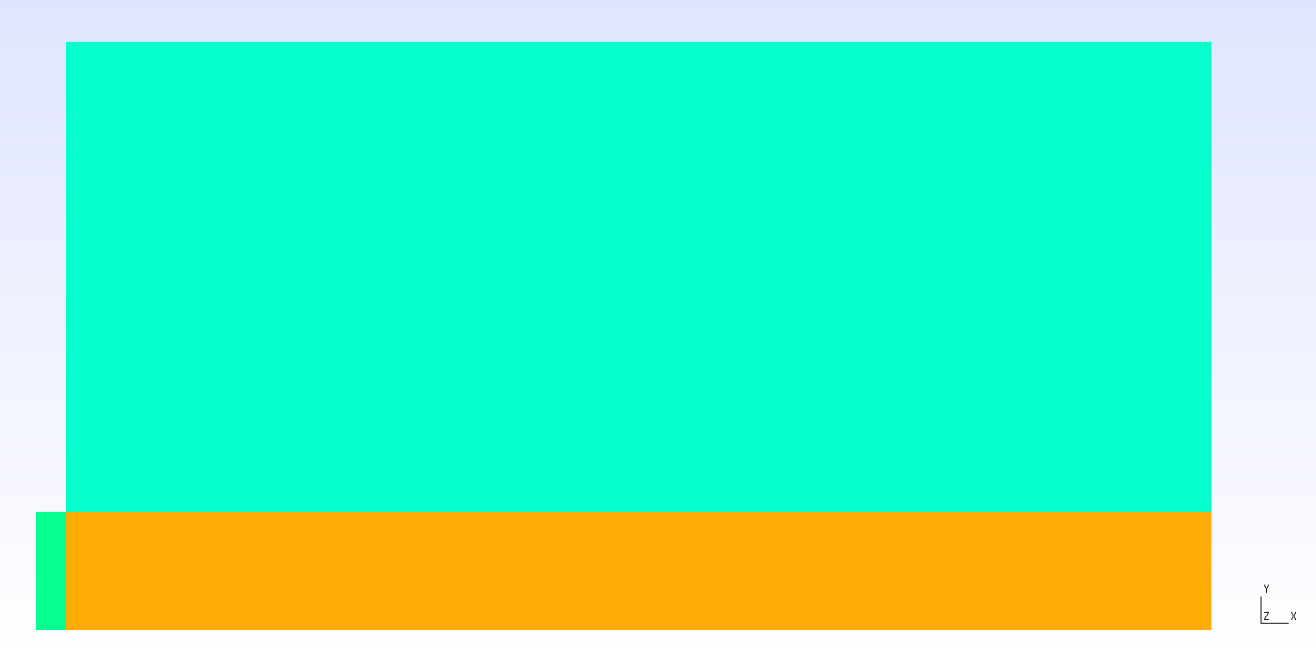
\includegraphics[scale=0.35]{downburstKim.png}
  \caption{Mesh used for the IJ downburst simulation}
  \label{fig:kimDownburst}
\end{figure}

Many tests were done in this mesh to mostly approximate the exact profiles shown in the reference papaer \cite{kim}, however there were reproducitibility issues when trying to match one to one with their simulation. Some of the papers consulted brought only snapshots of the flow at certain adimensionalized time steps, making it more troublesome to find the exact instants for comparison. Besides this remark about the time comparison, a behaviour not described by Kim, but noted by other studies [citation needed] was seen. When the main vortex generated by the IG reaches the ground it forms a high pressure pocket that generates a secondary vortex and "bounces" up the wind flow. Generating the secondary vortex is expected, however this upward movement seen wasn't described by Kim. In tables \ref{tb:kimVorticity} and \ref{tb:kimPressure} is shown some snapshots of the simulation at timesteps $T \in \{1,5,8,11\}$. 

\begin{table} \label{tb:kimVorticity}
  \begin{tabular}{cc} 
    \centering
    \num\putindeepbox[7pt]{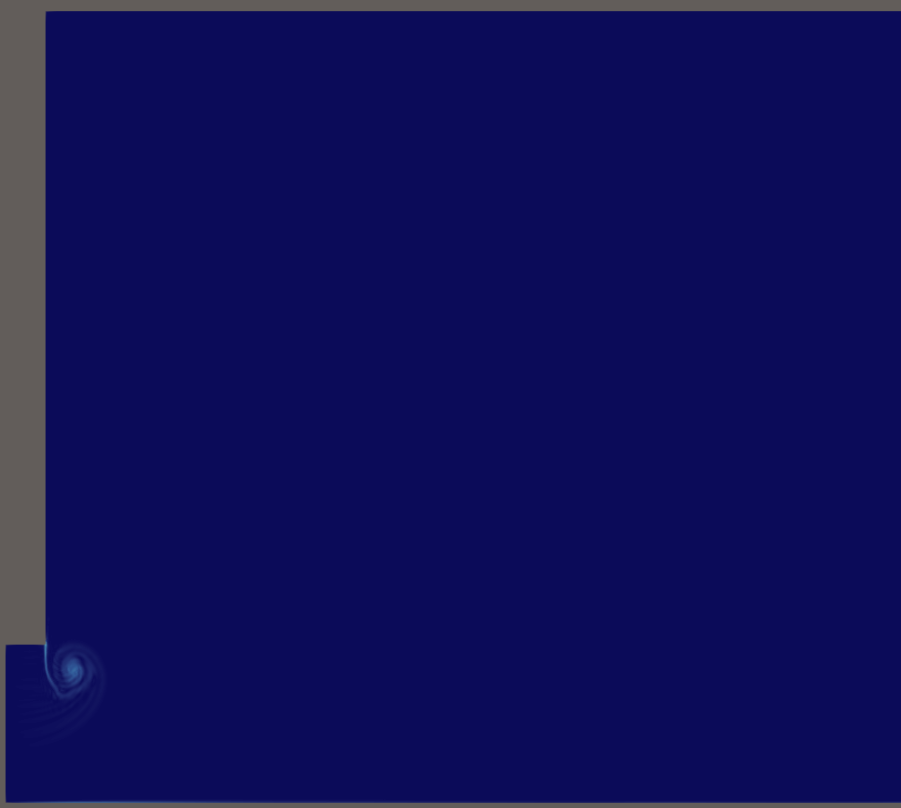
\includegraphics[scale=0.25]{kim0.png}}
      & \num\putindeepbox[7pt]{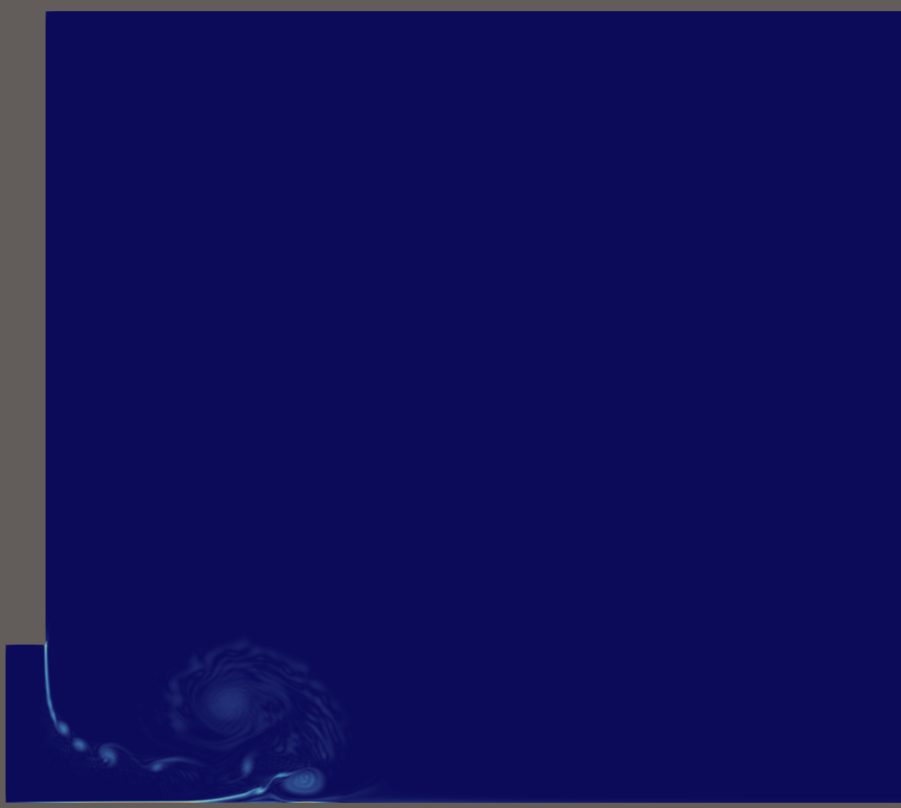
\includegraphics[scale=0.25]{kim4.png}} \\
    \num\putindeepbox[7pt]{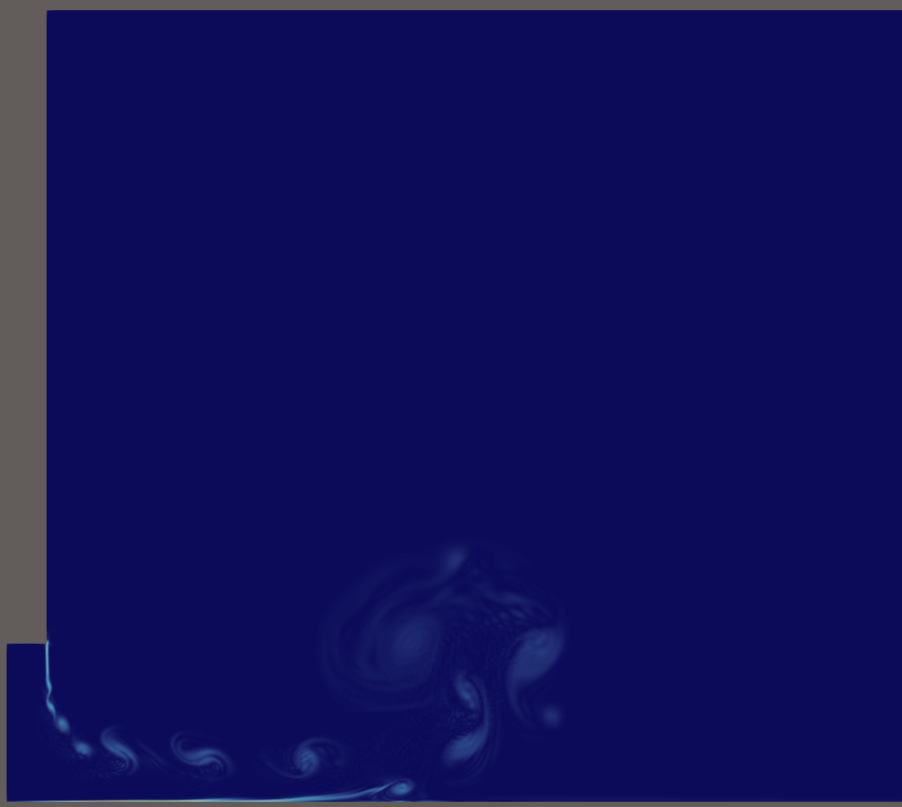
\includegraphics[scale=0.25]{kim7.png}}
      & \num\putindeepbox[7pt]{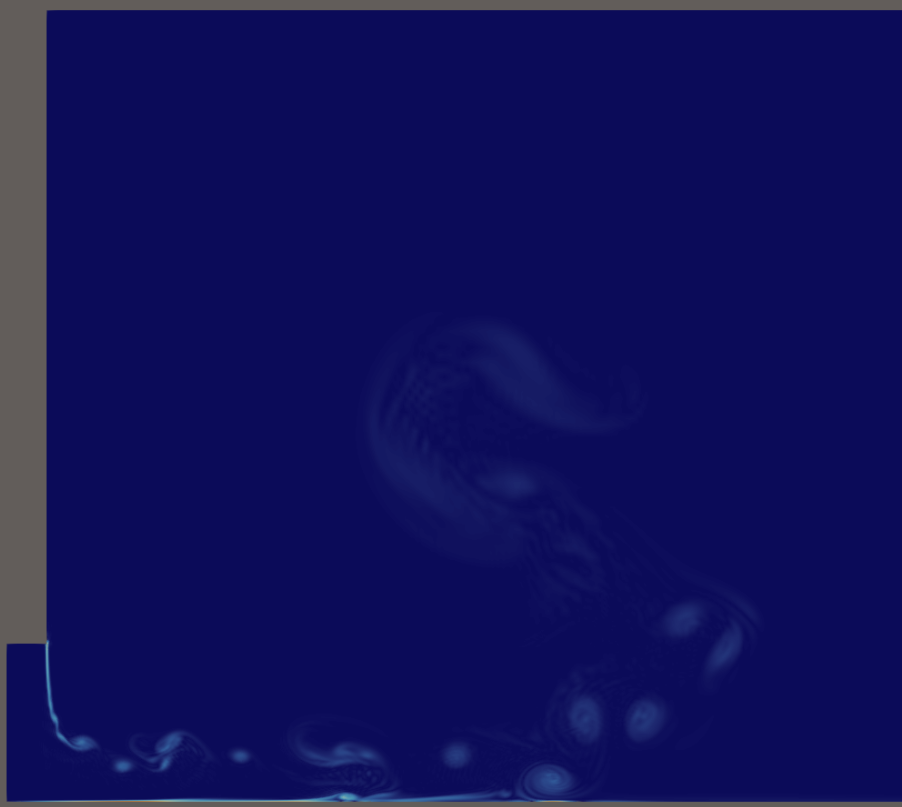
\includegraphics[scale=0.25]{kim11.png}} \\
  \end{tabular}
  \caption{Vorticity snapshots for $T \in \{1,5,8,11\}$}
\end{table}

\begin{table} \label{tb:kimPressure}
  \begin{tabular}{cc} 
    \centering
    \num\putindeepbox[7pt]{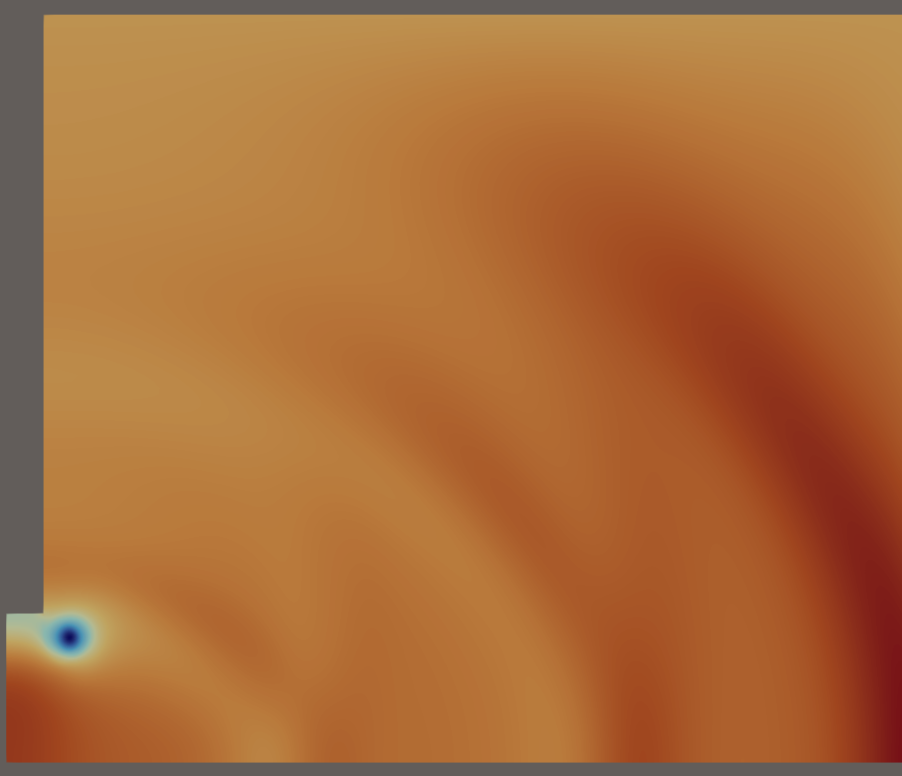
\includegraphics[scale=0.25]{kimp1.png}}
      & \num\putindeepbox[7pt]{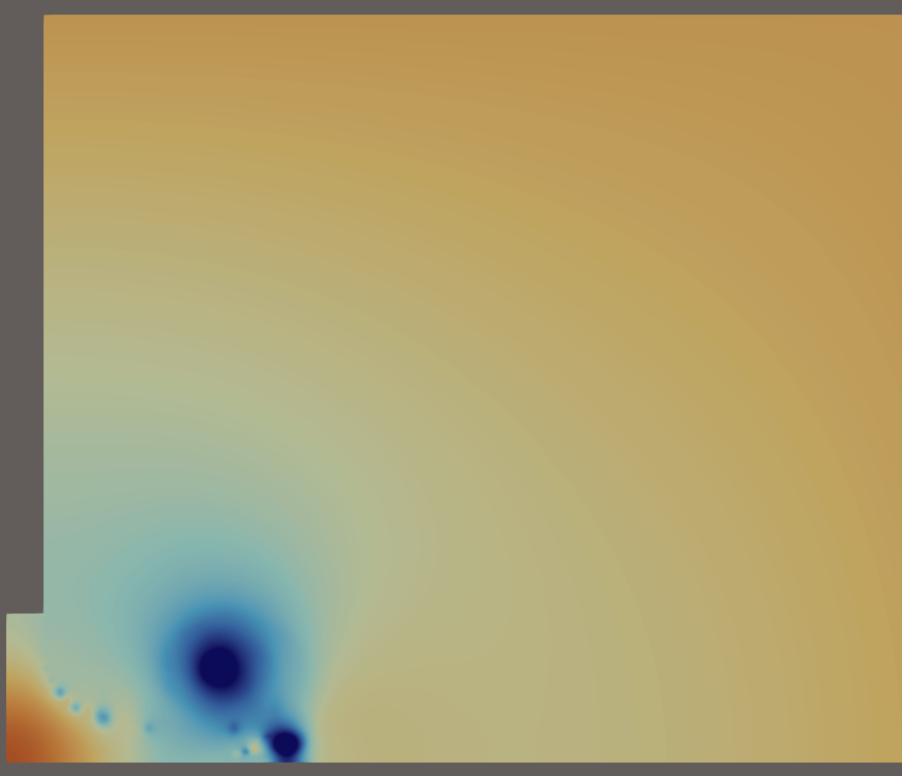
\includegraphics[scale=0.25]{kimp4.png}} \\
    \num\putindeepbox[7pt]{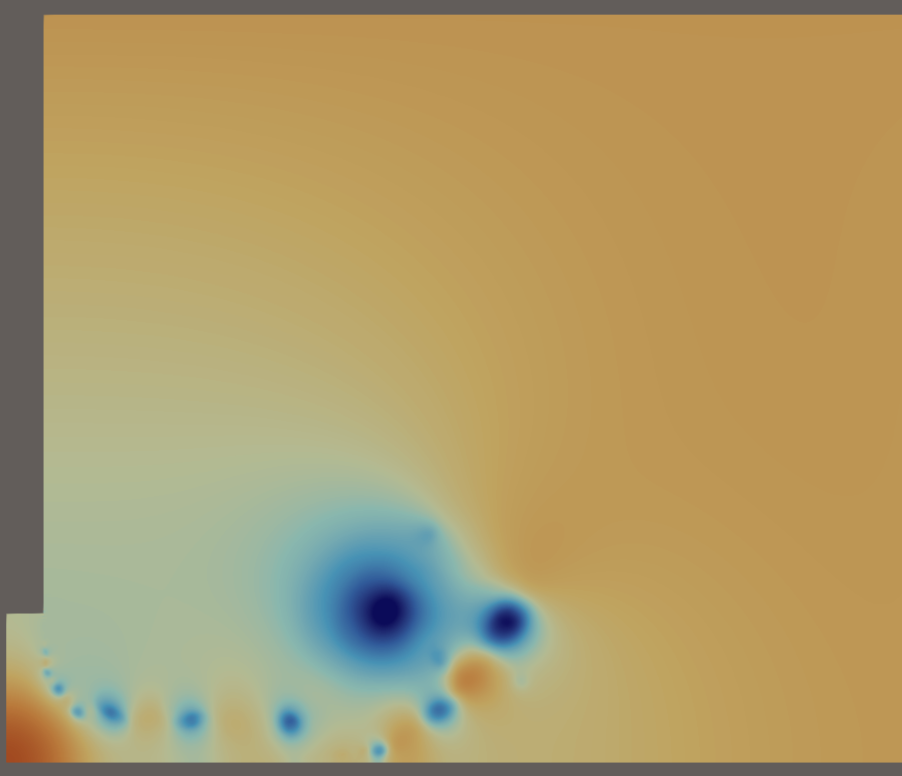
\includegraphics[scale=0.25]{kimp7.png}}
      & \num\putindeepbox[7pt]{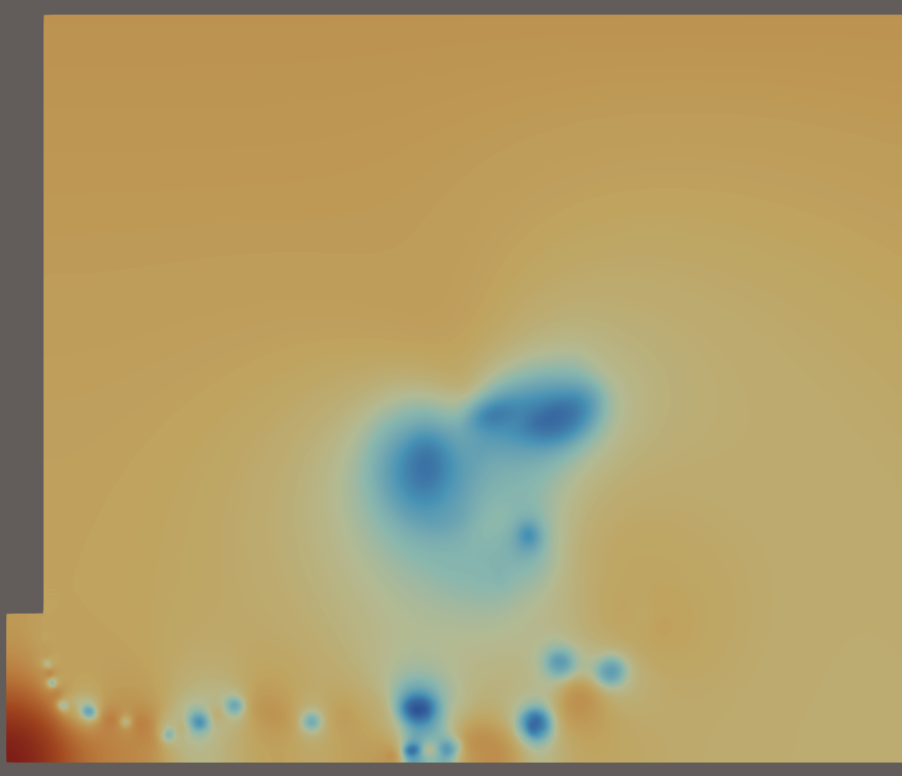
\includegraphics[scale=0.25]{kimp11.png}} \\
  \end{tabular}
  \caption{Pressure snapshots for $T \in \{1,5,8,11\}$}
\end{table}



\subsection{ABL on a Building} \label{abl}
\subsection{Downburst on A Building} \label{building}
\subsection{Simulation Results} \label{sim_results}
%
% Frame de campo de vorticidade e pressão, alguns frames, tipo cinco, perfis de velocidade
% LES, 2D, axissimétrico
%
\subsection{Performance Profiling of The GPU} \label{perf}
\section{Conclusion \& Further Discussion}
\section{Acknowledgments}


\bibliographystyle{ieeetr}
\bibliography{sample}

\end{document}
